\documentclass[a4paper,11pt]{article}

\usepackage[utf8]{inputenc}
\usepackage[T1]{fontenc}
\usepackage[spanish]{babel}
\usepackage[pdftex]{graphicx}
\usepackage[hyphens]{url}
\usepackage[pdftex]{hyperref}
\hypersetup{
	pdftitle={Reglamento Mini-Sumo},		% title
	pdfauthor={Club de Robótica FIUBA},	% author
	pdfsubject={Club de Robótica FIUBA},	% subject of the document
	colorlinks=true,		% false: boxed links;
	citecolor=black,		% color of links to bibliography
	filecolor=black,		% color of file links
	linkcolor=black,		% color of internal links
	urlcolor=black			% color of external links
}

%\usepackage{iwona}
\parskip=3pt
\headheight = 62pt

\usepackage{anysize}
%\marginsize{izquierdo}{derecho}{superior}{inferior}
\marginsize{2cm}{2cm}{1cm}{1cm}


\usepackage{fancyhdr}
\usepackage{lastpage}

%\fancyhf{} % clear all header and footer fields
\fancypagestyle{plain}{%
\fancyhead{} % get rid of headers
\renewcommand{\headrulewidth}{1pt} % and the line
\lhead{
\includegraphics[height=2cm]{logoclub}}
%\chead{}
\rhead{
\includegraphics[height=2cm]{logofiuba}}
\lfoot{ www.clubderobotica.com.ar}
\cfoot{}
\rfoot{ \thepage \ de \pageref{LastPage}}
}

\pagestyle{plain}

\let\oldenumerate\enumerate
\renewcommand{\enumerate}{
  \oldenumerate
  \setlength{\itemsep}{1pt}
  \setlength{\parskip}{0pt}
  \setlength{\parsep}{0pt}
}


\let\olditemize\itemize
\renewcommand{\itemize}{
  \olditemize
  \setlength{\itemsep}{1pt}
  \setlength{\parskip}{0pt}
  \setlength{\parsep}{0pt}
}

\usepackage{transparent}
\usepackage{eso-pic}
\newcommand\BackgroundPic{
  \put(0,0){
    \parbox[b][\paperheight]{\paperwidth}{%
      \vfill
      \centering
      {\transparent{0.05}
\includegraphics[width=0.9\paperwidth]{logoclub}}
      \vfill
    }
  }
}

\usepackage{wrapfig}

\newcommand{\cm}{\ensuremath{\mbox{~cm}}}
\newcommand{\mm}{\ensuremath{\mbox{~mm}}}
\newcommand{\gramos}{\ensuremath{\mbox{~g}}}

\newcommand{\dojo}{\emph{dohy\~{o}}~}

\author{Club de Robótica \\ Facultad de Ingeniería \\ Universidad de Buenos Aires}
\title{Competencia de Robótica 2014}


\begin{document}

\AddToShipoutPicture{\BackgroundPic}

\begin{center}
  {\Huge \textbf{Club de Robótica FIUBA}}
  \vspace{0.5cm}

  {\huge Competencia de Robótica 2014}
\end{center}


\section*{Objetivo de la competencia ``Mini-Sumo''}
El objetivo de la competición es diseñar y construir un robot que logre empujar al oponente fuera del \dojo.



\section*{Organización}
\subsection*{General}
\begin{itemize}
  \item La organización se reserva el derecho de introducir cualquier cambio en la normativa, cuando lo estime oportuno para el desarrollo de las pruebas.
  \item El jurado se conformará de 2 personas seleccionadas por los organizadores de la competencia.
  \item Las decisiones de los jueces serán, en todo momento, inapelables.
  \item Pueden participar de esta competencia cualquier persona interesada. De ser menor de 18 años debe asistir acompañado por un mayor responsable.
  \item Los organizadores se reservan el derecho de admisión. En caso de conductas inapropiadas, a criterio del jurado, los organizadores podrán excluir a los equipos involucrados.
\end{itemize}

\subsection*{Inscripción}
\begin{itemize}
  \item Cada robot podrá ser registrado (a través del formulario correspondiente) por un equipo de hasta 4 miembros.
  \item Cada robot llevará un nombre. En caso de que dos robots sean registrados con el mismo nombre, la prioridad está determinada por el orden de pre-inscripción. Los restantes equipos podrán seleccionar otro nombre, o simplemente agregar un identificador (por ejemplo: robot\_2).
  \item Cada equipo debe tener al menos 1 miembro mayor de 18 años, que será responsable por los miembros menores de edad que pueda tener el equipo.
  \item En el día de la competencia, por la mañana será la confirmación de asistencia y verificación de robots (``inscripción definitiva''). Es obligatorio presentarse antes de la finalización de este período para ser incluido en el torneo. Una vez cerrada la inscripción definitiva, se arma el cronograma de la competencia y orden de turnos, con todos los inscriptos.
  \item El horario de cierre de la ``inscripción definitiva'' se definirá en los días previos a la competencia. El horario de comienzo de la competencia se determinará el día del evento.
  \item Una vez publicado el orden, cada equipo es responsable de estar presente en el momento que corresponda su turno para competir.
  \item Parte de la calificación obtenida por los robots consiste en la documentación de cada robot debe presentar (ver ``El robot''). \textbf{Esta documentación debe ser enviada hasta una semana antes de la competencia}, de forma tal que el jurado tenga el suficiente tiempo para evaluarla.
  \item Además, esta información será publicada luego de finalizar la competencia, con el objetivo de favorecer el aprendizaje y fomentar el desarrollo de nuevos robots. Al realizar la inscripción del robot, todos los miembros del equipo están aceptando este compromiso.
\end{itemize}


\section*{El robot}
\subsection*{Requerimientos mínimos que debe cumplir el robot:}
\begin{itemize}
  \item El robot debe poseer un tamaño máximo de un cuadrado de $10\cm$ de lado, sin límite de altura.
  \item El peso máximo del robot es de $500\gramos$ (lo cual será verificado antes de cada combate).
  \item El robot debe diseñarse de forma que comience a moverse a partir de que reciba la señal de activación (ver abajo).
  \item El robot debe tener un interruptor (\emph{switch}) de seguridad que permita detenerlo inmediatamente. El interruptor debe ser visible y accesible quedando a criterio de los jueces el cumplimiento de este requerimiento.
  \item El robot debe ser completamente autónomo, es decir no podrá necesitar de ningún tipo de conexión o comunicación con el exterior para competir. Sí está permitido que el robot transmita datos útiles para el análisis de su desempeño. En caso de ser solicitado por el jurado, el equipo deberá demostrar que el robot puede funcionar sin este enlace activado.
  \item El robot deberá utilizar baterías. Está prohibido el uso de cualquier tipo de combustible.
  \item El robot puede desplegar estructuras una vez iniciado el asalto superando las restricciones de tamaño, pero sin separarse en 2 o más partes.
  \item El robot no puede tener ningún tipo de material o elementos que puedan dañar el \dojo y/o al oponente, quedando a criterio de los jueces el cumplimiento de este requerimiento.
\end{itemize}

\subsubsection*{Señal de activación}



\begin{itemize}
  \item El robot debe disponer de un acceso a tres señales: VCC, GPIO y GND.
  \item El acceso debe ser de, por lo menos, una de las dos siguientes formas.
  \begin{itemize}
    \item Un conector hembra de circuito impreso para tira de pines, de 3 posiciones, con el orden indicado (1-VCC 2-GPIO 3-GND).
    \item Un conector de tira de pines macho, de 3 posiciones, con el orden indicado (1-VCC 2-GPIO 3-GND).
  \end{itemize}
  \item En ambos casos debe estar claramente identificado el pin 1.
  \item La señal de activación será un flanco positivo en la línea GPIO. También podrá identificarse por la presencia de un nivel alto (``1 lógico'').
  \item La línea GPIO estará conectada a VCC a través de un resistor pull-up de 10 kohm y a GND a través de un transistor que actúa como llave (ver imagen). Cuando el transistor esté en modo saturación (llave cerrada) la línea GPIO presentará un ``0 lógico''.
  \begin{center}
    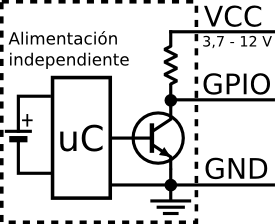
\includegraphics[width=0.3\textwidth]{signalstarter_sch}
  \end{center}
  \item Cuando el uC envíe la señal de activación, el transistor pasara al estado de corte (llave abierta) logrando de esta manera que la línea GPIO presente un ``1 lógico''.
  \item El nivel de tensión correspondiente al ``1 lógico'' depende de la tensión de alimentación provista por el robot en la línea VCC. Se sugiere conectar la línea GPIO a una entrada del micro tri-state, sin pull-up interno, de forma tal de no degradar la señal.
  \item El circuito del generador de señal de activación es auto alimentado, con lo cual el robot no debe proveer energía para dicho fin. El circuito solo presenta de carga la resistencia de pull-up mientras el transistor está en modo saturación (llave encendida). También hay que tener presente que mientras el transistor está en modo saturación, la línea GPIO presenta un camino de baja impedancia hacia GND.
  \item Se asegura que el la diferencia de tiempos máxima, de recepción de la señal por cada módulo será de 10 ms, caso contrario se reinicia el asalto.
  \item El tamaño según las indicaciones en la imagen son A: $25\mm$ - B: $53\mm$ - C: $33\mm$.
  \begin{center}
    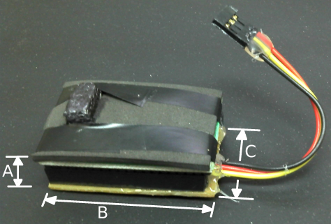
\includegraphics[width=0.3\textwidth]{signalstarter_img}
  \end{center}
  \item El peso es menor a $50\gramos$
  \item El peso del módulo no forma parte del peso del robot, es decir, el peso se verifica sin el módulo instalado.
\end{itemize}

No hay más restricciones, se pueden usar kits de robótica, kits de electrónica, o diseños completamente propios.

Se puede utilizar cualquier procesador o circuito para controlar el auto. El mismo criterio se aplica a los sensores, donde cualquiera está permitido.

Si bien no existen limitaciones para el largo del robot, y las referidas al ancho del robot son bastante laxas, se recomienda tener en cuenta las dimensiones de la pista ya que, por ejemplo, un robot muy grande quizás no pueda girar en las curvas más pronunciadas, o se caería fácilmente de la pista.

Sugerencias:
\begin{itemize}
  \item El robot puede optar por no utilizar el pull-up del generador de señal, en cuyo caso no será necesaria la línea VCC y queda a responsabilidad del robot el correcto establecimiento de los niveles lógicos (por medio de un circuito de pull-up en el robot).
  \item La señal de activación se mantendrá en el estado ``1 lógico'' durante todo el asalto. Se sugiere diseñar el robot para detenerse cuando reciba un flanco descendente en la línea GPIO o la presencia de un nivel bajo.
  \begin{center}
    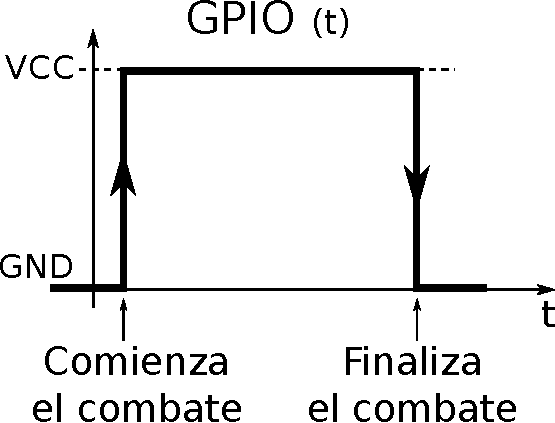
\includegraphics[width=0.3\textwidth]{signalstarter_tiempos}
  \end{center}
\end{itemize}


\subsection*{Documentación del robot}
Parte de la calificación del robot comprende la evaluación, por parte del jurado, de la documentación prevista por el equipo.
Dicha documentación debe incluir:
\begin{enumerate}
  \item Carátula: documento editable provisto por el Club (descargar en la página) 
  \item Introducción:
  \begin{itemize}
    \item Descripción básica del funcionamiento del robot 
    \item Objetivos (simpleza, excelencia, económico, reciclado, repetible, etc.)
  \end{itemize}
  \item Mecánica:
  \begin{itemize}
    \item Descripción de la estructura mecánica
    \item Especificaciones técnicas (Tipo, potencia y rpm de los motores, fuente de alimentación, etc.)
  \end{itemize}
  \item Electrónica:
  \begin{itemize}
    \item Descripción del circuito y mención de los integrados utilizados
    \item Esquemático y/o PCB 
  \end{itemize}
  \item Programación:
  \begin{itemize}
    \item Método de programación y programador utilizado
    \item Descripción de la lógica del código y lenguaje utilizado 
  \end{itemize}
  \item Conclusiones: Conclusiones del trabajo, costo total del robot, posibles mejoras a implementar, alternativas consideradas, etc.
  \item Anexo:
  \begin{itemize}
    \item Mecánica: Diagrama y planos (Diagramas 3d, dibujos, fotos del ensamblaje y/o croquis)
    \item Electrónica: Diagrama en bloques (optativo)
    \item Programación: 
    \begin{enumerate}
      \item Código fuente (en caso de que sea analógico, especificarlo, y explicar como calibraron el robot)
      \item Diagrama de flujos (optativo)
    \end{enumerate}
  \end{itemize}
\end{enumerate}

Las descripciones deben ser breves y concisas. La documentación no debe exceder el límite de 6 hojas máximo sin contar el anexo. 

El formato del documento deberá ser: 

Hoja: A4, Letra: Arial, Tamaño: 11, Alineación: Justificada, Interlineado: Sencillo y Sangría: $0.5\cm$. 

Se deberá enviar el archivo en formato PDF.

Un jurado puede solicitar a algunos participantes hacer una breve exposición oral e informal de los diseños luego de finalizar la carrera, ante toda la audiencia.

El objetivo de publicar los diseños y solicitar las presentaciones orales es favorecer el aprendizaje de todos los concursantes, estudiando los diseños de los demás.

Al momento de la inscripción, los miembros del equipo aseguran que la información presentada es de su propiedad intelectual, y/o los debidos créditos fueron incluidos. También acuerdan ceder los derechos de publicación de la información a los organizadores del evento, siendo ésta debidamente referenciada (es decir, aceptan que la información sea publicada en la página del club de robótica, indicando quiénes son los autores).


\section*{El área de combate}
\begin{itemize}
  \item El área de combate consiste del \dojo y del área exterior al \dojo
  \begin{center}
    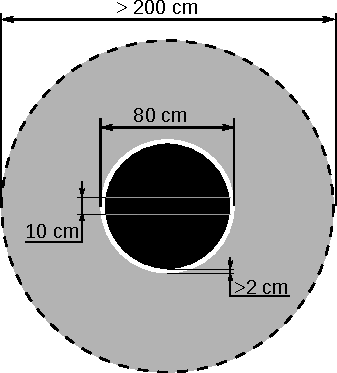
\includegraphics[width=0.3\textwidth]{doyho_mini_sumo}
  \end{center}
  \item El \dojo es un área circular de color negro, de 80 cm de diámetro.
  \item El límite del \dojo será delimitado por una línea blanca de 2 cm de ancho mínimo.
  \item El \dojo se encontrará elevado 2 cm respecto del suelo.
  \item El área exterior al \dojo será un círculo de por lo menos 2 metros de diámetro.
  \item En el centro del \dojo habrá dos líneas paralelas de color negro, separadas 10 cm, llamada líneas Shikiri.
\end{itemize}


\section*{La competencia}
\subsection*{Prueba de Homologación}
\begin{itemize}
  \item Los robots deberán superar una prueba que demuestre la capacidad de detectar y atacar al oponente.
  \item Esta prueba consiste en colocar al robot en el \dojo contra un oponente testigo cuyas dimensiones serán próximas a las requerimientos impuestos a los robots.
  \item El robot y el testigo se colocarán en posiciones aleatorias y el robot dispondrá de 90 segundos para detectar y sacarlo del \dojo.
  \item Durante la homologación también se valida el funcionamiento de la activación remota.
  \item El robot puede intentar la homologación tantas veces como lo desee, siempre que los tiempos de la organización lo permitan, hasta el inicio de la competencia.
\end{itemize}

\subsection*{Combate}
\subsubsection*{General}
\begin{itemize}
\item Para el comienzo del combate se llamarán a los dos equipos participantes.
\item Se realizarán como máximo tres avisos con un intervalo de 1 minuto entre ellos, y si en el plazo de 1 minuto desde el último aviso uno de los equipos no se presentara, se otorgará la victoria al otro equipo.
\item Si, en el caso extremo ningún equipo se presentara, los jueces tendrán la facultad de declarar el combate sin vencedor, o determinar la espera de, como máximo, otros 5 minutos. Una vez finalizado este período se declarará el combate sin vencedor y dependiendo de la instancia de la competencia, los equipos podrán ser descalificados.
\item Cada equipo designará un responsable del equipo.
\item Cada combate contará con la presencia de un árbitro que se encargará de dar inicio al combate e interactuar con los responsables de cada equipo.
\item El combate consiste de 3 asaltos.
\item Entre asaltos habrá un tiempo máximo de 1 minuto.
\item Durante todo el combate, incluido el minuto entre asaltos, sólo el responsable del equipo podrá entrar en el área de combate.
\item Cuando los jueces den por finalizado el combate, los responsables de cada equipo retirarán los robots del área de combate.
\item El robot que gane la mayor cantidad de asaltos gana el combate.
\item Si luego de 3 asaltos ningún robot obtuvo una diferencia respecto del otro, los jueces podrán determinar el método de conclusión del combate.
\end{itemize}

\subsubsection*{Asalto}
\begin{itemize}
\item El asalto tiene una duración máxima de 3 minutos.
\item El responsable del equipo situará el robot en el \dojo.
\item En principio, los robots se situarán en cualquier parte del semicírculo delimitado por la línea \emph{Shikiri} y el borde blanco del ring.
\item Los jueces determinarán, en cada asalto, la posición y orientación inicial de los robots.
\item En el caso de que los jueces determinen que la orientación y/o posición inicial es libre, se sorteará qué equipo posiciona primero el robot.
\item El juez accionará el sistema de activación, que enviará un mensaje a cada módulo, los cuales generarán la señal de activación.
\item Cuando los robots están compitiendo en un asalto nadie podrá entrar en el área de combate. Únicamente se podrá acceder dentro de este área cuando el combate esté paralizado.
\item Los jueces podrán detener el asalto cuando lo consideren necesario, para permitir, si fuera necesario, la entrada de los responsables de cada equipo al área de combate.
\item Si el asalto se detiene antes de que haya pasado 1 minuto de los 3 máximos, se volverá a empezar inmediatamente desde las posiciones de inicio (reiniciando el tiempo del asalto).
\item Cada asalto podrá reiniciarse hasta 2 ocasiones. Si el asalto debiera detenerse por tercera vez, el asalto se declara empatado, salvo que los jueces consideren apropiado reiniciar nuevamente el asalto.
\item Si el asalto se detiene luego de que haya pasado 1 minuto de los 3 máximos, el asalto se declara empatado.
\end{itemize}

El asalto se termina con un vencedor cuando:
\begin{itemize}
\item El robot oponente es el primero en tocar el suelo fuera del \dojo.
\item El robot oponente pierde una pieza o se separa en 2 o más partes.
\item El robot oponente comete 2 violaciones.
\end{itemize}

Nota: el módulo de activación no forma parte del robot, y su desprendimiento del robot no es considerado una falta. Además, en dicho caso, el asalto se reiniciará.

Si durante uno de los asaltos uno de los robots resulta dañado (desprendimiento de piezas), el equipo afectado podrá solicitar por única vez en el combate 5 minutos adicionales de pausa para intentar subsanar la anomalía. Si en ese tiempo no se resuelve el problema se dará por finalizado el combate, resultando vencedor el otro equipo. Queda a decisión de los jueces la concesión de los 5 minutos adicionales.

El asalto se detendrá cuando:
\begin{itemize}
\item Los dos robots permanezcan 15 segundos sin moverse.
\item Los dos robots permanezcan 30 segundos sin tocarse.
\item Los dos robots permanezcan 45 segundos empujándose pero sin que el movimiento favorezca a ninguno de los equipos.
\item Alguno de los dos robots pierde el módulo de señal de activación.
\item Se produzca una violación al reglamento.
\end{itemize}

Se consideran violaciones:
\begin{itemize}
\item Que el robot despliegue alguna estructura antes que se haya enviado la señal de acitvación.
\item Que el responsable del equipo entre en el área de combate sin autorización previa del árbitro.
\item Que un equipo tarde más de 30 segundos en volver a empezar el combate después de se haya detenido.
\end{itemize}

Se considerará penalización (implicando la pérdida del combate):
\begin{itemize}
\item Que cualquier miembro del equipo que no sea el responsable, entre en el área de combate.
\item Que un equipo supere el minuto entre asalto y asalto sin solicitud previa.
\item Que un robot provoque desperfectos en el \dojo.
\item Que el robot se fije al \dojo mediante dispositivos de succión, pegamentos, etc.
\item Que el robot utilice dispositivos que lancen líquido, polvo, gases o sólidos al oponente.
\item Que un robot utilice dispositivos inflamables.
\item Que un robot o un miembro del equipo cause desperfectos de forma deliberada al oponente.
\end{itemize}

\subsection*{Puntuación}
Se calificará a los robots en tres categorías
\begin{enumerate}
  \item Resultado de la carrera (P1): se asignará un puntaje entre 0 y 10 puntos, según la siguiente escala:
  \begin{itemize}
    \item 10 puntos para el primero.
    \item  8 puntos para el segundo.
    \item  6 puntos para el tercero.
    \item  4 puntos para el cuarto.
    \item  2 puntos para los restantes robots que completaron una vuelta.
    \item  0 puntos para los que no completaron una vuelta del circuito.
  \end{itemize}    
    Se entiende por ``primero'' aquel robot que completa la vuelta en menor tiempo.

  \item Documentación (P2): El jurado calificará con una escala de 0 a 5 puntos la documentación presentada por cada equipo.
  A criterio del jurado se evaluará la calidad y completitud de todos los items indicados en la sección documentación.

  \item Originalidad del Robot (P3): El jurado calificará de 0 a 5 puntos según la originalidad que consideren de cada robot.
\end{enumerate}

Se dispondrá de una evaluación de cada jurado en relación a las categorías 2 y 3. Para cada una de estas categorías se promedian todos los puntajes otorgados por los jurado. Por ejemplo, para la categoría P2 se tendrán las notas de los 3 jurados. P2 se calcula como:

\begin{center}
P2=(J1+J2+J3)/3
\end{center}

La puntuación final del robot se obtiene con la siguiente ecuación:

\begin{center}
Puntaje final = P1 $\cdot$ $0.5$ + P2 $\cdot$ $0.7$ + P3 $\cdot$ $0.3$
\end{center}

Está ecuación junto con las escalas seleccionadas otorga pesos a cada categoría de la siguiente forma:

1) 50\%  2) 35\%  3) 15\%

La puntuación máxima posible es 10 puntos.

\textbf{El ganador de la competencia es el robot que obtenga mayor cantidad de puntos}.

\noindent\rule{\textwidth}{0.4pt}

Este reglamento fue confeccionado por los miembros del Club de Robótica utilizando como base los siguientes reglamentos:
\begin{enumerate}
  \item Grupo de Robótica UTN - Bahía Blanca - Competencia sumo: \\
        \url{http://www.grsbahiablanca.com.ar/compe_2012.htm}
\end{enumerate}



















\end{document}
